\documentclass[a4paper]{article}
\usepackage[utf8]{inputenc}
\usepackage[english]{babel}
\usepackage[T1]{fontenc}
\usepackage{lmodern}
\usepackage{fullpage}
\usepackage{amsmath}
\usepackage{graphicx}
\usepackage{framed}
\usepackage{listings}
\usepackage{placeins}
\usepackage{subcaption}
\usepackage{array}
\usepackage{mathtools}
\usepackage{hyperref}
\usepackage{mhchem}
\usepackage[justification=centering]{caption}

\title{Computational Methods for \\Systems and Synthetic Biology:\\ Project report}
\author{Théotime Grohens}

\begin{document}
\maketitle

\section{Introduction}

For this project, we reimplemented the cellular model described in \cite{weisse}.
It is a very simple ordinary differential equation (ODE) model, which allows us to reimplement and change it easily.
After a brief description of the model, we study the influence of nutrient efficiency and the effect of adding chloramphenicol into the medium on cell growth.
Then, we show that the model is able to describe gene dosage compensation behaviors in cells, and we finally study the consequences of adding a toggle switch circuit into the cell.

\section{Description of the model}

The model focuses on the trade-offs that all cells must face when they grow, in their allocation of resources: they have finite levels of energy, and thus must regulate transcription (the main energy consumer in the cell); they have a finite amount of ribosomes, so they must pick which genes to translate in order to balance mRNAs; and, finally, they have a finite mass, so they must also balance the different levels of proteins.
The model is coarse-grained, meaning that it aims at describing this behavior with minimal complexity.

The behavior of the cell is ruled by 14 different variables: an internal nutrient $s_i$, a general-purpose energy source $a$ made from the nutrient, and the protein, mRNA and ribosome-mRNA complex levels of 4 different kinds of proteins: a transporter enzyme $e_t$ that imports an external nutrient into the internal nutrient, a metabolic enzyme $e_m$ that turns the internal nutrient into energy, ribosomes $r$ and an umbrella \emph{housekeeping} protein $q$ that comprises all other proteins found in the cell.

The model is described as a set of elementary chemical reactions involving these species; these boil down to a set of ordinary differential equations describing the evolutions of their concentrations over time.

\section{Influence of nutrient efficiency and chloramphenicol presence}

\begin{figure}[h]
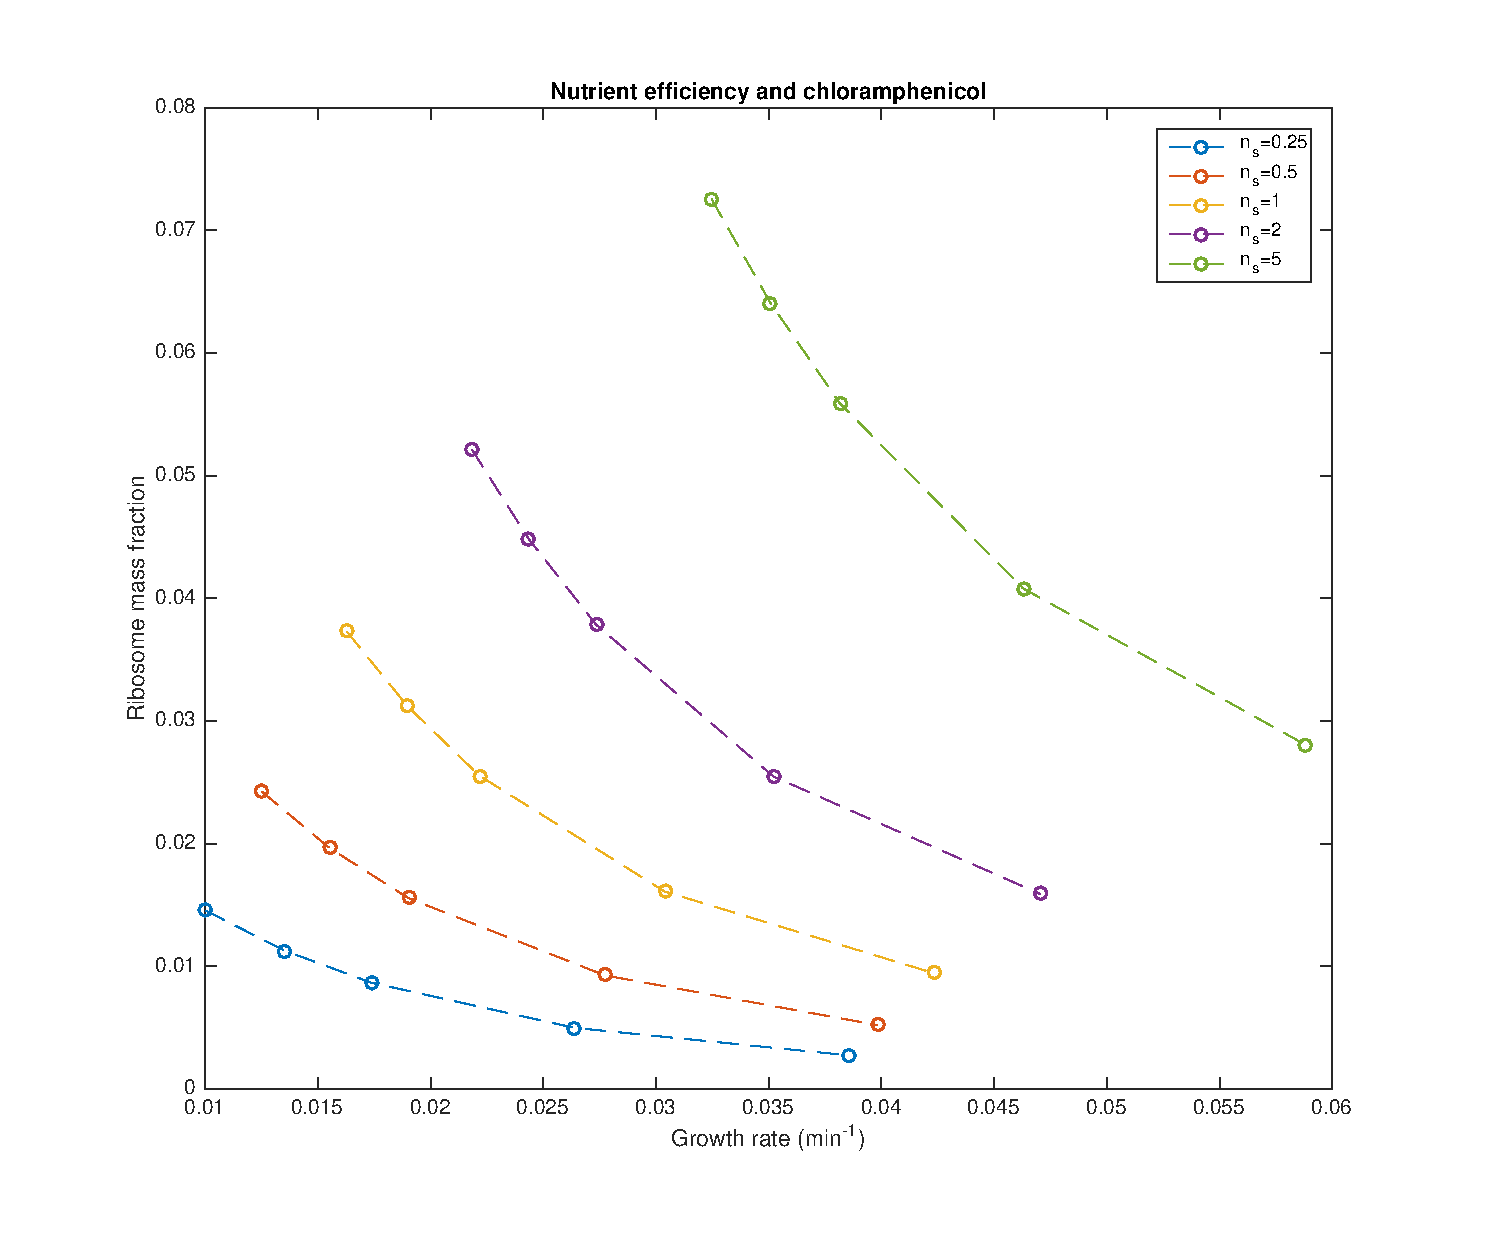
\includegraphics[width=\textwidth]{chlor.eps}
\caption{Influence of varying nutrient efficiency and chloramphenicol concentration on growth rate and ribosome mass fraction.}
\label{chlor}
\end{figure}

Nutrient efficiency $n_s$ is a parameter that describes the efficiency of the metabolic enzyme $e_m$ at turning the internal nutrient $s_i$ into energy $a$.
It appears in this equation: $s_i \xrightarrow[]{\nu_{cat}}n_sa$, with $\nu_{cat}$, the catalysis rate, depending on $e_m$.
Efficiency is a parameter that can model the well-adaptedness of the metabolic processes in the cell with regard to their environment.
Varying this high-level parameter can model changes in the external medium. 

Chloramphenicol is an antibiotic that binds to mRNA-ribosome complexes, and inhibits their translation as well as the release of the ribosome from the complex.
The inactivated \emph{zombie} complexes can then only disappear from the cell through dilution.

The paper studies the evolution of ribosome mass fraction and cell growth at either constant chloramphenicol levels and varying nutrient efficiencies, or at constant nutrient efficiency and varying chloramphenicol levels.
At constant nutrient efficiency, there is a positive correlation between cell growth and ribosome mass fraction, while this correlation is negative at constant chloramphenicol.

This can be explained as the consequence of the energy trade-off: with more available energy, the cell can afford to have more ribosomes, and will grow faster (translate more), because translation is the only process that costs the cell energy in the model.

However, when we increase chloramphenicol levels, ribosomal efficiency is reduced since chloramphenicol binds to the (mRNA-bound) ribosomes and renders them useless.
Thus, a higher ribosomal mass fraction just means that more of the protein mass is useless, which hinders the cell's growth.

\FloatBarrier

\section{Transcription rates and energy levels}

\begin{figure}[h]
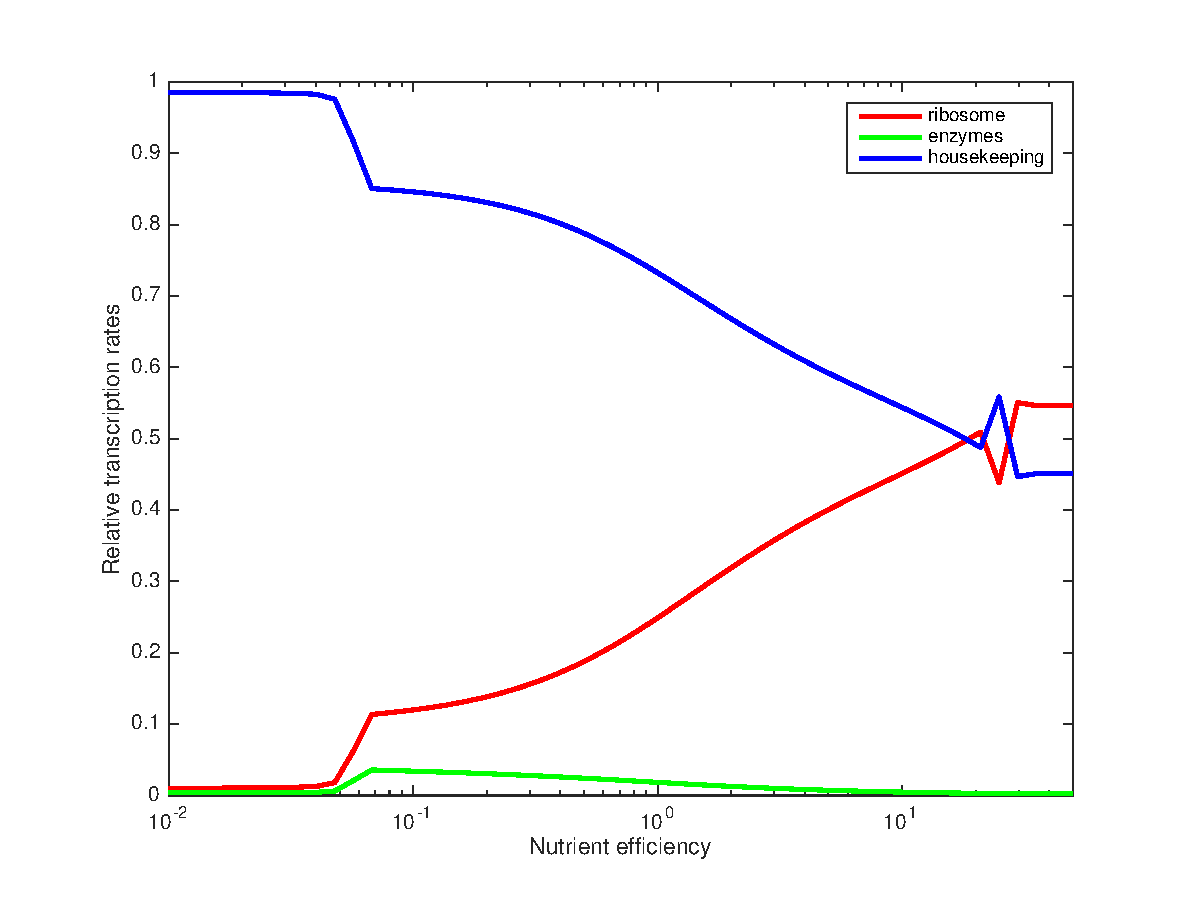
\includegraphics[width=\textwidth]{transcription.eps}
\caption{Evolution of transcription rates with nutrient efficiency.}
\label{trans}
\end{figure}

In this section, we look at the final transcription rates of the different kinds of proteins with varying nutrient efficiencies.
The different transcription thresholds of the proteins lead to different evolution of the translation rates.
At low available energy, the cell produces less ribosomes but more enzymes than at higher energies, which causes more enzymes to be produced, and thus more energy to be imported into the cell.

Conversely, at higher available energies, the cell can afford to have more ribosomes,which is costly because they need translating, but which helps translate more of all proteins.
The figure \ref{trans} describes this evolution and matches the one in the paper, although it plots transcription rates directly against nutrient efficiency because the available energy in the cell $a$ is not a parameter of the system.

\section{Gene dosage compensation}

\begin{figure}[h]

\begin{subfigure}{0.5\textwidth}
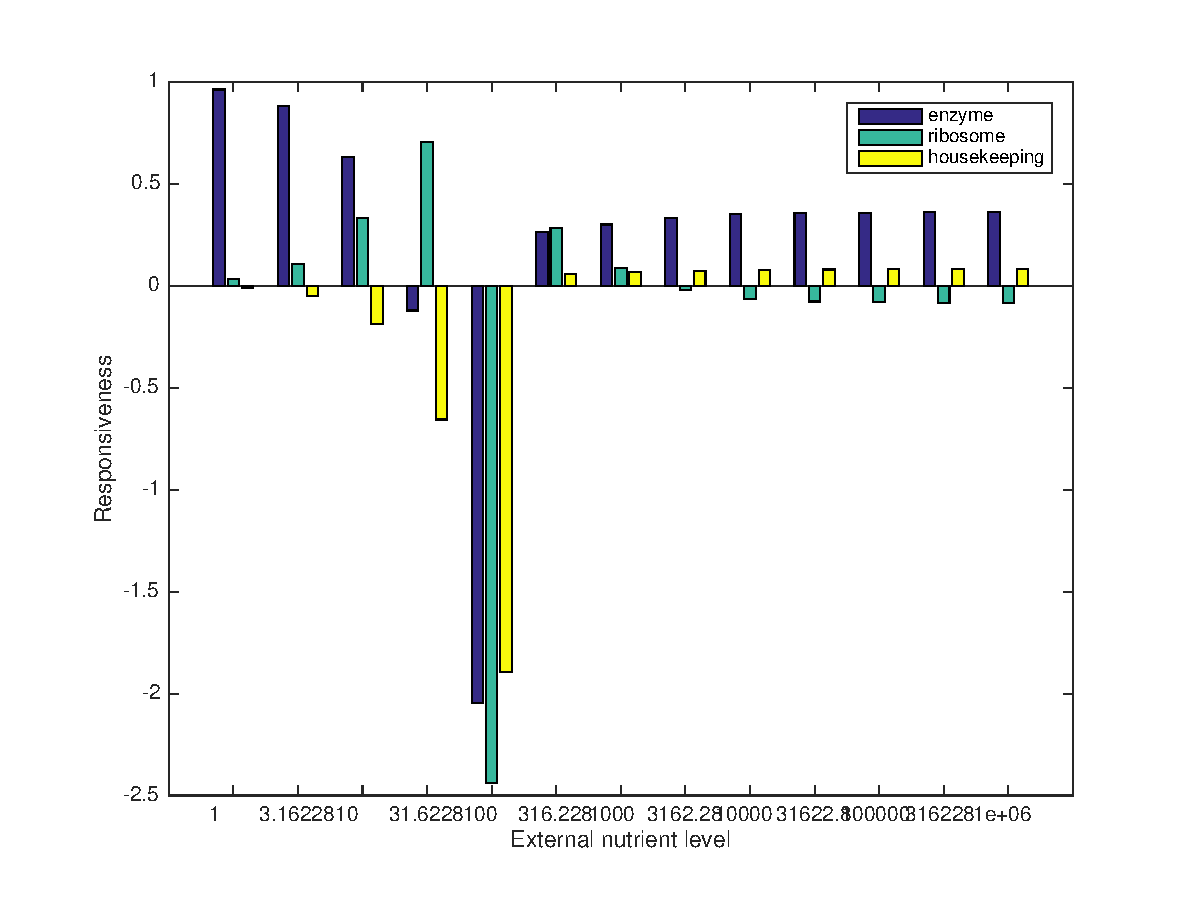
\includegraphics[width=\textwidth]{enzdel.eps}
\caption{Responsiveness in the enzyme deletion strain.}
\label{enzdel}
\end{subfigure}
\begin{subfigure}{0.5\textwidth}
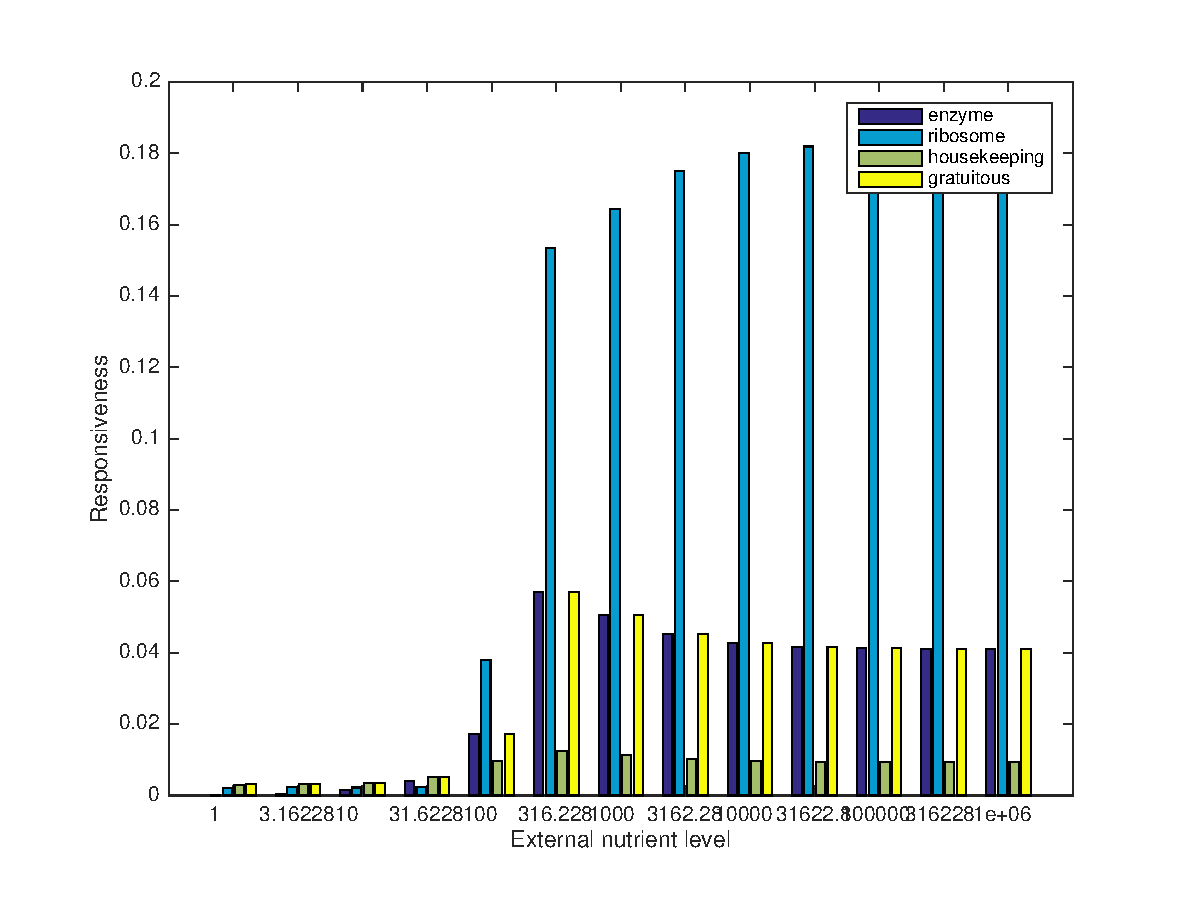
\includegraphics[width=\textwidth]{gratdel.eps}
\caption{Responsiveness in the gratuitous protein deletion strain.}
\label{gratdel}
\end{subfigure}

\centering
\begin{subfigure}{0.49\textwidth}
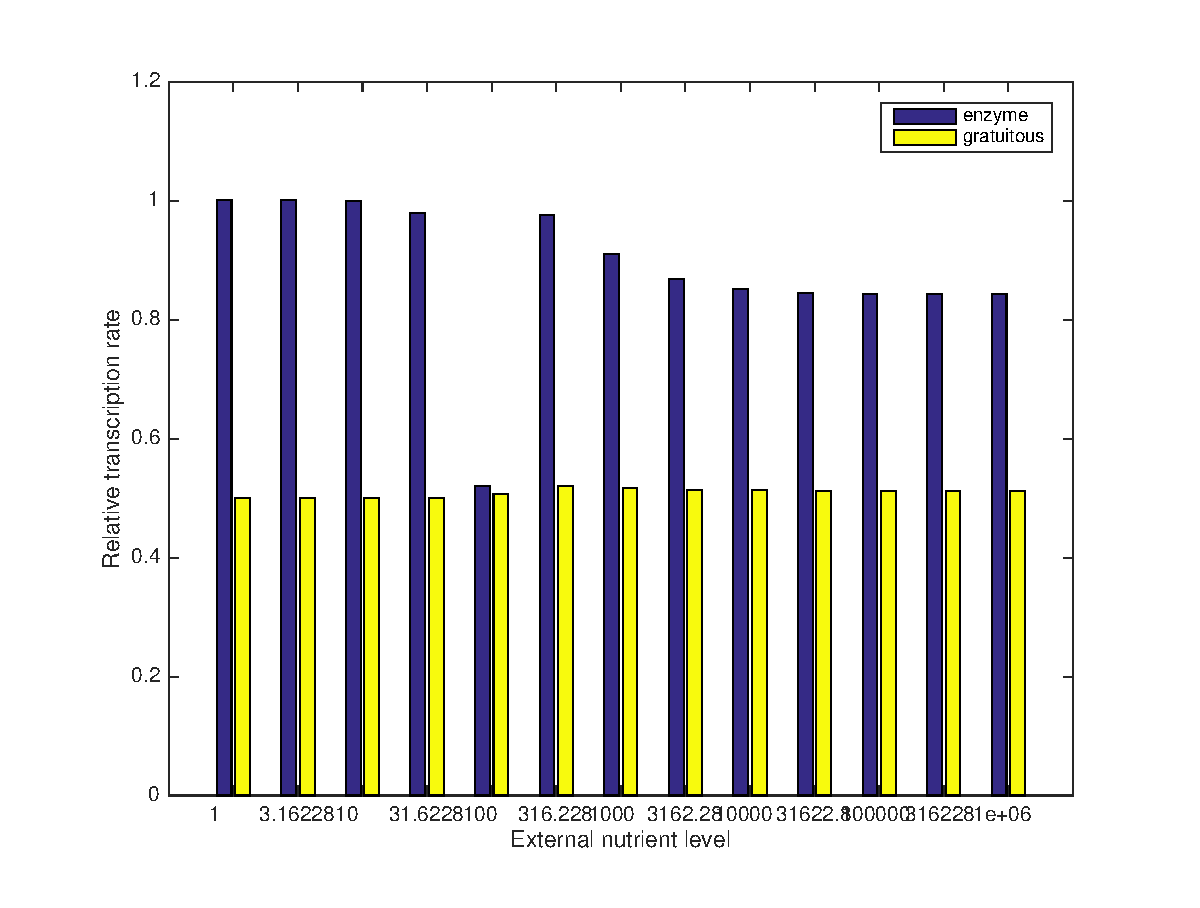
\includegraphics[width=\textwidth]{reltransdel.eps}
\caption{Relative transcription rates in the deletion strains.}
\label{reltransdel}
\end{subfigure}

\caption{Gene dosage compensation for an enzyme deletion and a gratuitous protein deletion.}
\label{resp}
\end{figure}

Gene dosage compensation is a phenomenon that can affect cells that have two copies of the same (or paralogous) gene.
If one of the copies of the gene is deactivated (for example, due to a random mutation), we can sometimes observe that the expression level of the other copy is not half the expression level of the gene when its two copies are expressed.
This indicates that there is a feedback loop on the expression levels of this gene.

In the paper, the authors simulate both an enzyme deletion strain (by dividing maximal transcription rates by 2), and a gratuitous protein deletion strain.
The gratuitous protein is modelled by a new set of differential equations that mimics the other ones, except that the protein plays no role in the cell metabolism, and has no retroaction loop on its expression rate (unlike the housekeeping proteins).
It can thus help model what happens when an external synthetic circuit is inserted into a cell, but does not interact with its metabolism other than by consuming energy for translation.

The responsiveness is a measure of the gene dosage compensation effect; it is the logarithm of the ratio of expression levels in the wild-type strain and the deletion strain, for each kind of protein.
A responsiveness of 0 indicates that there is no compensation; a positive responsiveness indicates that the cell expresses more of the remaining gene in order to compensate for the loss of one of the copies, and a negative responsiveness indicates on the contrary that the gene is even less expressed.
Since the expression of a gene can influence the expression levels of other genes, we also measure the responsiveness of other genes to the deletion of one of the paralogous genes.

We compute responsiveness at different levels of external nutrient (and not nutrient efficiency), in order to see which trade-offs the cells will have to make based on the environment they live in.

In the enzyme deletion strain, we can see a positive responsiveness for enzymes, which indicates that the cell does try to maintain enzyme levels.
However, as the quantity of nutrient increases, the responsiveness for ribosomes turns negative; this means that it is at the cost of expressing ribosomes that the cell expresses more enzymes.
The negative peak is probably due to the differential equation integrating that results in erroneous results, since they differ from those in the paper.

In the gratuitous protein deletion strain, all responsivenesses are positive.
This result shows that when the cell can express less of the gratuitous protein, it can devote a larger part of its energy to its own processes, rather than making the protein.
However, the responsivenesses are lower in absolute value than in the enzyme deletion strain, which means that the cell is less sensitive to a variation of the expression level of the gratuitous protein (that does not play a role in its metabolism), rather than to a variation of the enzyme expression levels.


\FloatBarrier

\section{Toggle switch}

\begin{figure}[h]
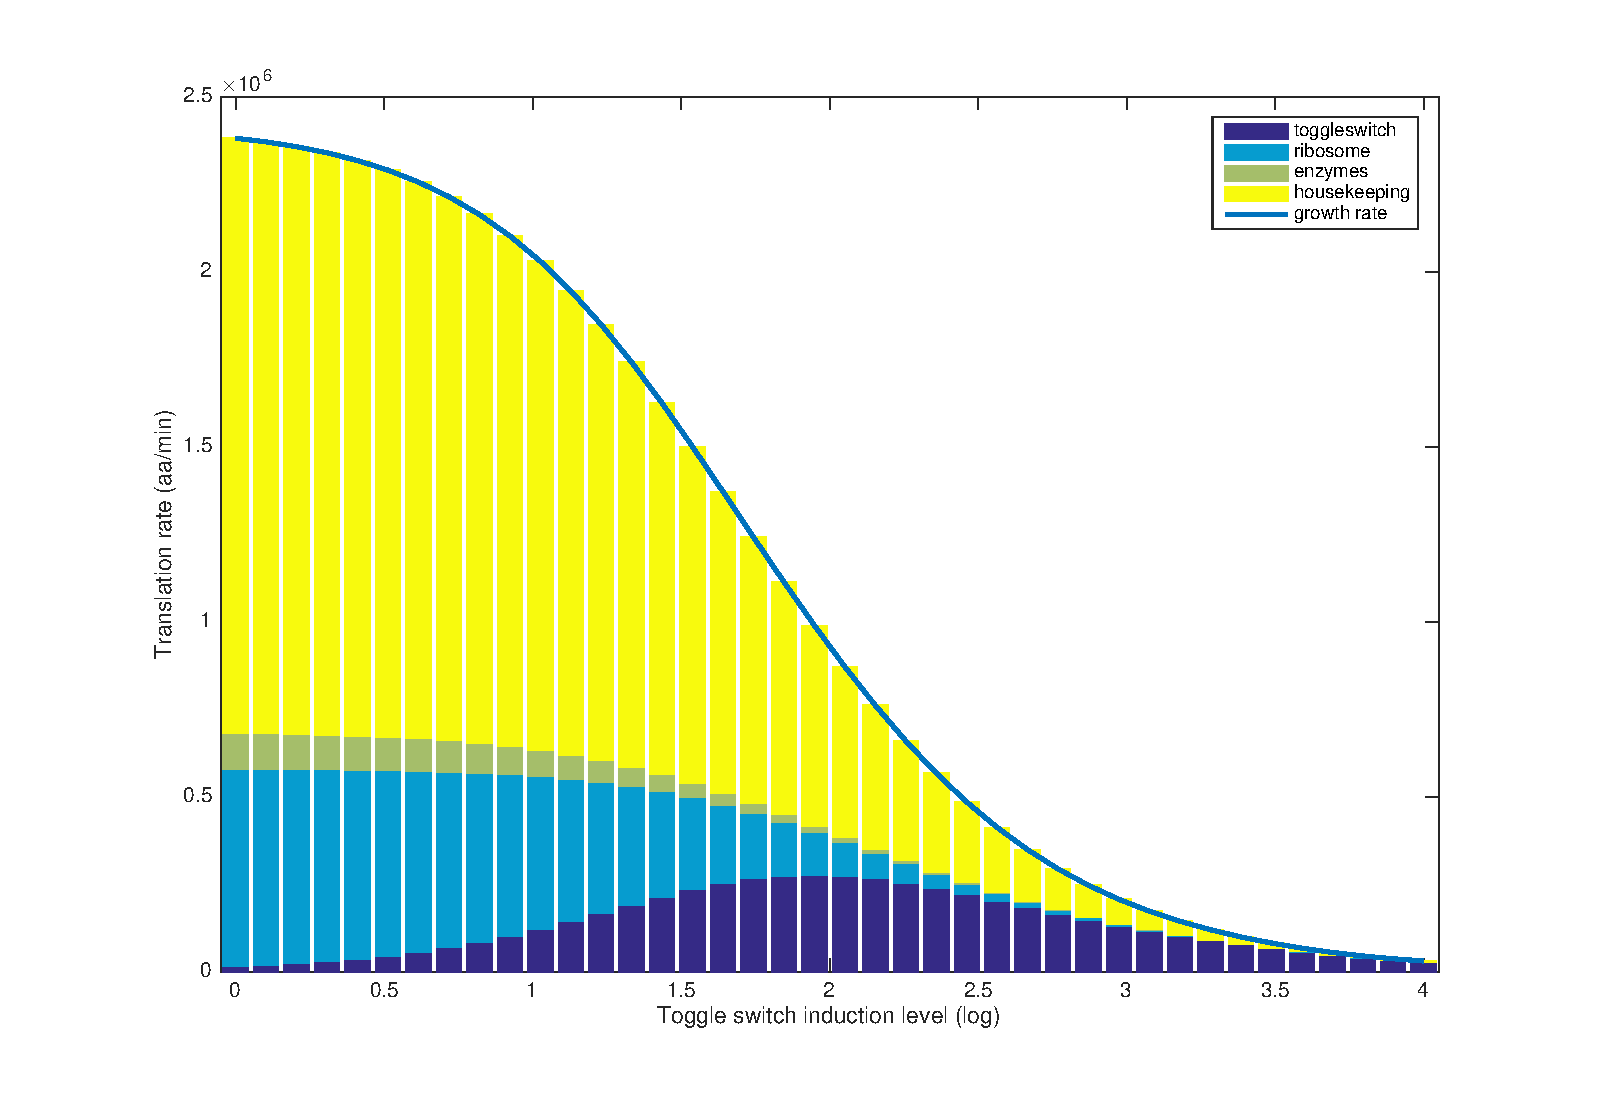
\includegraphics[width=\textwidth]{induction.eps}
\caption{Protein transcription rates and cell growth rate (in min$^{-1}$)}
\end{figure}

The toggle switch is an example of a synthetic circuit that can be inserted into a cell, in order to study both its functioning inside that particular cell but also the reaction of the cell to the addition of this new element.
Although the original paper used a repressilator, which does not converge to a steady state but goes through periodic cycles, we implemented a toggle switch because it is conceptually simpler, but interact the same way with the cell.

In this experiment, we are interested in how the toggle switch affects the normal functioning of the cell, so we simulate adding the genes for LacI and TetR at the steady state of the base model, and then run the simulation until we reach steady state again.

The parameter that we change is the induction level of the switch: indeed, what is interesting when adding a new synthetic circuit to a cell is to see how much it impacts the normal functioning of the cell, in order for example to maximize production of some chemical species.

At low induction levels, the toggle switch uses up a very small fraction of the cell's translation resources (free ribosomes), and so has little impact.
However, as induction grows, the proportion of ribosomes used by the switch increases, which leads to decreased production of the other kinds of proteins (especially the housekeeping proteins), and to a decreased cell growth rate as well.
Finally, when induction reaches too high levels, the toggle switch takes too important a toll on the cell's resources, and the absolute level of translation of the switch begins to decrease again, until cell growth reaches a stop when the circuit takes up all of the cell's ribosomes.

This figure shows the same behavior as the one in the original paper, which uses a repressilator instead of a toggle switch.
This confirms the idea that as long as the circuit does not directly interact with the rest of the cell's metabolism, the details of the circuit itself are irrelevant, and only its induction levels (and more generally the proportion of the cell's resources that it uses) are relevant.

\FloatBarrier

\begin{thebibliography}{9}
	\bibitem {weisse} Andrea Y. Weiße, Diego A. Oyarz\'un, Vincent Danos, Peter S. Swain. \emph{A mechanistic link between cellular trade-offs, gene expression and growth}. In \emph{Proc. Natl. Acad. Sci. USA}, E1038-E1047, February 2015. 
\end{thebibliography}

\end{document}